% =====================================================================
%  REPORT — CSRF Attack on Elgg via the Fetch API (English)
%  Compile: xelatex report_en.tex  (run 2-3 times for the ToC)
% =====================================================================
\documentclass[11pt,a4paper]{article}

\usepackage{fontspec}
\setmainfont{TeX Gyre Termes}
\setsansfont{TeX Gyre Heros}
\setmonofont{Noto Sans Mono}[Scale=0.86]

\usepackage[english]{babel}

\usepackage[a4paper,margin=2.4cm,headheight=15pt]{geometry}
% =====================================================================
%  sty_common.tex — Shared visual style for the CSRF report (VI / EN)
%  Engine: XeLaTeX. Input AFTER \documentclass, fontspec fonts and babel.
% =====================================================================

% ---------- Colours (tie-in with the exploit page palette) -----------
\usepackage{xcolor}
\definecolor{navy}{HTML}{1E3C72}
\definecolor{brandblue}{HTML}{2A5298}
\definecolor{accent}{HTML}{2563EB}
\definecolor{danger}{HTML}{DC2626}
\definecolor{success}{HTML}{15803D}
\definecolor{amber}{HTML}{B45309}
\definecolor{ink}{HTML}{0F172A}
\definecolor{slate}{HTML}{475569}
\definecolor{mist}{HTML}{F1F5F9}
\definecolor{line}{HTML}{CBD5E1}
\definecolor{codebg}{HTML}{0F172A}
\definecolor{codefg}{HTML}{E2E8F0}
\definecolor{codekey}{HTML}{38BDF8}
\definecolor{codestr}{HTML}{86EFAC}
\definecolor{codecom}{HTML}{94A3B8}

% ---------- Graphics / diagrams --------------------------------------
\usepackage{graphicx}
\usepackage{tikz}
\usetikzlibrary{arrows.meta,positioning,calc,shadows.blur,backgrounds,fit}

% ---------- Tables ---------------------------------------------------
\usepackage{booktabs}
\usepackage{array}
\usepackage{tabularx}
\usepackage{colortbl}
\newcolumntype{Y}{>{\raggedright\arraybackslash}X}
\newcolumntype{C}{>{\centering\arraybackslash}X}

% ---------- Callout boxes --------------------------------------------
\usepackage[most]{tcolorbox}

\newtcolorbox{infobox}[1][]{
  enhanced, breakable, colback=mist, colframe=accent,
  boxrule=0pt, leftrule=3pt, arc=2pt, left=10pt, right=10pt,
  top=7pt, bottom=7pt, fonttitle=\bfseries\color{navy},
  coltitle=navy, title={#1}}

\newtcolorbox{warnbox}[1][]{
  enhanced, breakable, colback=danger!6, colframe=danger,
  boxrule=0pt, leftrule=3pt, arc=2pt, left=10pt, right=10pt,
  top=7pt, bottom=7pt, fonttitle=\bfseries, coltitle=danger, title={#1}}

\newtcolorbox{okbox}[1][]{
  enhanced, breakable, colback=success!6, colframe=success,
  boxrule=0pt, leftrule=3pt, arc=2pt, left=10pt, right=10pt,
  top=7pt, bottom=7pt, fonttitle=\bfseries, coltitle=success, title={#1}}

% ---------- Source-code listings (JS / Python / HTTP / bash) ---------
\usepackage{listings}
\lstset{
  basicstyle=\footnotesize\ttfamily\color{codefg},
  backgroundcolor=\color{codebg},
  keywordstyle=\color{codekey}\bfseries,
  stringstyle=\color{codestr},
  commentstyle=\color{codecom}\itshape,
  numberstyle=\tiny\color{codecom},
  frame=single, framerule=0pt, rulecolor=\color{codebg},
  numbers=left, numbersep=8pt, tabsize=2,
  showstringspaces=false, breaklines=true, breakatwhitespace=false,
  columns=fullflexible, keepspaces=true,
  xleftmargin=14pt, xrightmargin=6pt, aboveskip=10pt, belowskip=6pt,
  % Mono font (Noto Sans Mono) has full Vietnamese coverage -> no literate hacks.
  extendedchars=true, inputencoding=utf8,
}
% JavaScript dialect
\lstdefinelanguage{JavaScript}{
  keywords={const,let,var,function,async,await,return,try,catch,new,if,else,
            for,while,of,in,typeof,this,null,true,false,window,document},
  morekeywords=[2]{fetch,URLSearchParams,FormData,append,addEventListener},
  keywordstyle=[2]\color{codestr}\bfseries,
  sensitive=true,
  morecomment=[l]{//}, morecomment=[s]{/*}{*/},
  morestring=[b]', morestring=[b]", morestring=[b]`,
}
\lstdefinestyle{http}{
  language={}, morekeywords={POST,GET,HTTP,Host,Cookie,Content-Type,User-Agent,Accept,Connection},
}

% ---------- Icons via dingbats (no fontawesome dependency) -----------
\usepackage{pifont}
\newcommand{\yes}{\textcolor{success}{\ding{52}}}
\newcommand{\no}{\textcolor{danger}{\ding{56}}}
\newcommand{\step}[1]{\textcolor{white}{\colorbox{accent}{\footnotesize\bfseries~#1~}}}

% ---------- Misc -----------------------------------------------------
\usepackage{enumitem}
\setlist{leftmargin=1.4em,itemsep=2pt,topsep=3pt}
\usepackage{microtype}


\usepackage{fancyhdr}
\usepackage{titlesec}
\usepackage{lastpage}
\usepackage{hyperref}
\hypersetup{colorlinks=true,linkcolor=accent,urlcolor=accent,citecolor=accent,
  pdftitle={CSRF Attack on Elgg via the Fetch API},
  pdfauthor={Group 6 - Computer Security}}

% ---- Section styling ----
\titleformat{\section}{\sffamily\Large\bfseries\color{navy}}{\thesection.}{0.6em}{}[{\color{line}\titlerule[1pt]}]
\titleformat{\subsection}{\sffamily\large\bfseries\color{brandblue}}{\thesubsection}{0.6em}{}
\titleformat{\subsubsection}{\sffamily\normalsize\bfseries\color{ink}}{\thesubsubsection}{0.6em}{}
\titlespacing*{\section}{0pt}{16pt}{8pt}

% ---- Header / footer ----
\pagestyle{fancy}
\fancyhf{}
\fancyhead[L]{\footnotesize\sffamily\color{slate}CSRF on Elgg · Fetch API}
\fancyhead[R]{\footnotesize\sffamily\color{slate}Computer Security — Group 6}
\fancyfoot[C]{\footnotesize\sffamily\color{slate}Page \thepage{} / \pageref{LastPage}}
\renewcommand{\headrulewidth}{0.4pt}
\renewcommand{\headrule}{\hbox to\headwidth{\color{line}\leaders\hrule height \headrulewidth\hfill}}

% ---- English labels for the shared sequence diagram ----
\newcommand{\lblVictim}{Alice (victim) + Browser}
\newcommand{\lblAttacker}{Attacker\\\texttt{attacker.csrf.localhost}}
\newcommand{\lblElgg}{Elgg\\\texttt{elgg.csrf.localhost}}
\newcommand{\lblSa}{1. Legitimate login}
\newcommand{\lblSb}{2. Set-Cookie \texttt{Elgg=...}}
\newcommand{\lblSc}{3. Accidentally opens malicious page}
\newcommand{\lblSd}{4. Returns \texttt{index.html} (Fetch script)}
\newcommand{\lblNe}{5. Script auto-runs (\texttt{DOMContentLoaded})}
\newcommand{\lblSf}{6. Fetch POST + cookie (\texttt{credentials:'include'})}
\newcommand{\lblNg}{7. Valid cookie $\Rightarrow$ About me updated}
\newcommand{\lblSh}{8. Response 302 (opaque)}
\newcommand{\lblSi}{9. Reload profile $\to$ it was changed}
% =====================================================================
%  diagram_flow.tex — CSRF attack sequence diagram (\csrfflowdiagram)
%  Labels default to Vietnamese; an English document may \renewcommand
%  them BEFORE % =====================================================================
%  diagram_flow.tex — CSRF attack sequence diagram (\csrfflowdiagram)
%  Labels default to Vietnamese; an English document may \renewcommand
%  them BEFORE % =====================================================================
%  diagram_flow.tex — CSRF attack sequence diagram (\csrfflowdiagram)
%  Labels default to Vietnamese; an English document may \renewcommand
%  them BEFORE \input{diagram_flow}.
% =====================================================================
\providecommand{\lblVictim}{Alice (nạn nhân) + Trình duyệt}
\providecommand{\lblAttacker}{Attacker\\\texttt{attacker32.com}}
\providecommand{\lblElgg}{Elgg\\\texttt{seed-server.com}}
\providecommand{\lblSa}{1. Đăng nhập hợp lệ}
\providecommand{\lblSb}{2. Set-Cookie \texttt{Elgg=...}}
\providecommand{\lblSc}{3. Vô tình mở trang độc hại}
\providecommand{\lblSd}{4. Trả \texttt{index.html} (Fetch script)}
\providecommand{\lblNe}{5. Script tự chạy (\texttt{DOMContentLoaded})}
\providecommand{\lblSf}{6. Fetch POST + cookie (\texttt{credentials:'include'})}
\providecommand{\lblNg}{7. Cookie hợp lệ $\Rightarrow$ cập nhật About me}
\providecommand{\lblSh}{8. Phản hồi 302 (opaque)}
\providecommand{\lblSi}{9. Xem lại hồ sơ $\to$ đã bị đổi}

\newcommand{\csrfflowdiagram}{%
\begin{tikzpicture}[
   >={Stealth[length=2.4mm]}, font=\sffamily\scriptsize,
   head/.style={draw=navy,fill=navy,text=white,rounded corners=3pt,
                align=center,minimum height=0.85cm,minimum width=3.2cm,
                font=\sffamily\scriptsize\bfseries},
   life/.style={line,dashed,line width=0.7pt},
   msg/.style={->,accent,line width=0.9pt},
   ret/.style={->,slate,line width=0.7pt,dashed},
   note/.style={draw=amber,fill=amber!12,rounded corners=2pt,align=center,
                inner sep=3pt,font=\sffamily\scriptsize,text=amber!60!black}]

  \def\ax{0} \def\bx{5.4} \def\cx{10.8}
  \def\ytop{0} \def\ybot{-9.3}

  % lifeline heads
  \node[head] (A) at (\ax,\ytop) {\lblVictim};
  \node[head] (B) at (\bx,\ytop) {\lblAttacker};
  \node[head] (C) at (\cx,\ytop) {\lblElgg};

  % lifelines
  \draw[life] (\ax,-0.55) -- (\ax,\ybot);
  \draw[life] (\bx,-0.55) -- (\bx,\ybot);
  \draw[life] (\cx,-0.55) -- (\cx,\ybot);

  % messages
  \draw[msg] (\ax,-1.2) -- node[above]{\lblSa} (\cx,-1.2);
  \draw[ret] (\cx,-2.0) -- node[above]{\lblSb} (\ax,-2.0);
  \draw[msg] (\ax,-2.9) -- node[above]{\lblSc} (\bx,-2.9);
  \draw[ret] (\bx,-3.7) -- node[above]{\lblSd} (\ax,-3.7);

  \node[note,anchor=north west] at (\ax-1.7,-4.35) {\lblNe};

  \draw[msg,danger] (\ax,-5.6) -- node[above,text=danger]{\lblSf} (\cx,-5.6);

  \node[note,anchor=north] at (\cx,-6.2) {\lblNg};

  \draw[ret] (\cx,-7.4) -- node[above]{\lblSh} (\ax,-7.4);
  \draw[msg,success] (\ax,-8.4) -- node[above,text=success]{\lblSi} (\cx,-8.4);
\end{tikzpicture}%
}
.
% =====================================================================
\providecommand{\lblVictim}{Alice (nạn nhân) + Trình duyệt}
\providecommand{\lblAttacker}{Attacker\\\texttt{attacker32.com}}
\providecommand{\lblElgg}{Elgg\\\texttt{seed-server.com}}
\providecommand{\lblSa}{1. Đăng nhập hợp lệ}
\providecommand{\lblSb}{2. Set-Cookie \texttt{Elgg=...}}
\providecommand{\lblSc}{3. Vô tình mở trang độc hại}
\providecommand{\lblSd}{4. Trả \texttt{index.html} (Fetch script)}
\providecommand{\lblNe}{5. Script tự chạy (\texttt{DOMContentLoaded})}
\providecommand{\lblSf}{6. Fetch POST + cookie (\texttt{credentials:'include'})}
\providecommand{\lblNg}{7. Cookie hợp lệ $\Rightarrow$ cập nhật About me}
\providecommand{\lblSh}{8. Phản hồi 302 (opaque)}
\providecommand{\lblSi}{9. Xem lại hồ sơ $\to$ đã bị đổi}

\newcommand{\csrfflowdiagram}{%
\begin{tikzpicture}[
   >={Stealth[length=2.4mm]}, font=\sffamily\scriptsize,
   head/.style={draw=navy,fill=navy,text=white,rounded corners=3pt,
                align=center,minimum height=0.85cm,minimum width=3.2cm,
                font=\sffamily\scriptsize\bfseries},
   life/.style={line,dashed,line width=0.7pt},
   msg/.style={->,accent,line width=0.9pt},
   ret/.style={->,slate,line width=0.7pt,dashed},
   note/.style={draw=amber,fill=amber!12,rounded corners=2pt,align=center,
                inner sep=3pt,font=\sffamily\scriptsize,text=amber!60!black}]

  \def\ax{0} \def\bx{5.4} \def\cx{10.8}
  \def\ytop{0} \def\ybot{-9.3}

  % lifeline heads
  \node[head] (A) at (\ax,\ytop) {\lblVictim};
  \node[head] (B) at (\bx,\ytop) {\lblAttacker};
  \node[head] (C) at (\cx,\ytop) {\lblElgg};

  % lifelines
  \draw[life] (\ax,-0.55) -- (\ax,\ybot);
  \draw[life] (\bx,-0.55) -- (\bx,\ybot);
  \draw[life] (\cx,-0.55) -- (\cx,\ybot);

  % messages
  \draw[msg] (\ax,-1.2) -- node[above]{\lblSa} (\cx,-1.2);
  \draw[ret] (\cx,-2.0) -- node[above]{\lblSb} (\ax,-2.0);
  \draw[msg] (\ax,-2.9) -- node[above]{\lblSc} (\bx,-2.9);
  \draw[ret] (\bx,-3.7) -- node[above]{\lblSd} (\ax,-3.7);

  \node[note,anchor=north west] at (\ax-1.7,-4.35) {\lblNe};

  \draw[msg,danger] (\ax,-5.6) -- node[above,text=danger]{\lblSf} (\cx,-5.6);

  \node[note,anchor=north] at (\cx,-6.2) {\lblNg};

  \draw[ret] (\cx,-7.4) -- node[above]{\lblSh} (\ax,-7.4);
  \draw[msg,success] (\ax,-8.4) -- node[above,text=success]{\lblSi} (\cx,-8.4);
\end{tikzpicture}%
}
.
% =====================================================================
\providecommand{\lblVictim}{Alice (nạn nhân) + Trình duyệt}
\providecommand{\lblAttacker}{Attacker\\\texttt{attacker32.com}}
\providecommand{\lblElgg}{Elgg\\\texttt{seed-server.com}}
\providecommand{\lblSa}{1. Đăng nhập hợp lệ}
\providecommand{\lblSb}{2. Set-Cookie \texttt{Elgg=...}}
\providecommand{\lblSc}{3. Vô tình mở trang độc hại}
\providecommand{\lblSd}{4. Trả \texttt{index.html} (Fetch script)}
\providecommand{\lblNe}{5. Script tự chạy (\texttt{DOMContentLoaded})}
\providecommand{\lblSf}{6. Fetch POST + cookie (\texttt{credentials:'include'})}
\providecommand{\lblNg}{7. Cookie hợp lệ $\Rightarrow$ cập nhật About me}
\providecommand{\lblSh}{8. Phản hồi 302 (opaque)}
\providecommand{\lblSi}{9. Xem lại hồ sơ $\to$ đã bị đổi}

\newcommand{\csrfflowdiagram}{%
\begin{tikzpicture}[
   >={Stealth[length=2.4mm]}, font=\sffamily\scriptsize,
   head/.style={draw=navy,fill=navy,text=white,rounded corners=3pt,
                align=center,minimum height=0.85cm,minimum width=3.2cm,
                font=\sffamily\scriptsize\bfseries},
   life/.style={line,dashed,line width=0.7pt},
   msg/.style={->,accent,line width=0.9pt},
   ret/.style={->,slate,line width=0.7pt,dashed},
   note/.style={draw=amber,fill=amber!12,rounded corners=2pt,align=center,
                inner sep=3pt,font=\sffamily\scriptsize,text=amber!60!black}]

  \def\ax{0} \def\bx{5.4} \def\cx{10.8}
  \def\ytop{0} \def\ybot{-9.3}

  % lifeline heads
  \node[head] (A) at (\ax,\ytop) {\lblVictim};
  \node[head] (B) at (\bx,\ytop) {\lblAttacker};
  \node[head] (C) at (\cx,\ytop) {\lblElgg};

  % lifelines
  \draw[life] (\ax,-0.55) -- (\ax,\ybot);
  \draw[life] (\bx,-0.55) -- (\bx,\ybot);
  \draw[life] (\cx,-0.55) -- (\cx,\ybot);

  % messages
  \draw[msg] (\ax,-1.2) -- node[above]{\lblSa} (\cx,-1.2);
  \draw[ret] (\cx,-2.0) -- node[above]{\lblSb} (\ax,-2.0);
  \draw[msg] (\ax,-2.9) -- node[above]{\lblSc} (\bx,-2.9);
  \draw[ret] (\bx,-3.7) -- node[above]{\lblSd} (\ax,-3.7);

  \node[note,anchor=north west] at (\ax-1.7,-4.35) {\lblNe};

  \draw[msg,danger] (\ax,-5.6) -- node[above,text=danger]{\lblSf} (\cx,-5.6);

  \node[note,anchor=north] at (\cx,-6.2) {\lblNg};

  \draw[ret] (\cx,-7.4) -- node[above]{\lblSh} (\ax,-7.4);
  \draw[msg,success] (\ax,-8.4) -- node[above,text=success]{\lblSi} (\cx,-8.4);
\end{tikzpicture}%
}


\begin{document}
\selectlanguage{english}

% =====================================================================
%  TITLE PAGE
% =====================================================================
\begin{titlepage}
\begin{tikzpicture}[remember picture,overlay]
  \fill[navy] (current page.north west) rectangle ([yshift=-5.2cm]current page.north east);
  \fill[brandblue] ([yshift=-5.2cm]current page.north west) rectangle ([yshift=-5.7cm]current page.north east);
  \node[anchor=north west,text=white,font=\sffamily\small] at ([xshift=2.4cm,yshift=-1.1cm]current page.north west)
     {VIETNAM NATIONAL UNIVERSITY, HANOI — UNIVERSITY OF SCIENCE};
  \node[anchor=north west,text=white,font=\sffamily\small] at ([xshift=2.4cm,yshift=-1.7cm]current page.north west)
     {Course: Computer Security};
  \node[anchor=north west,text=white,font=\sffamily\bfseries\LARGE,text width=16cm] at ([xshift=2.4cm,yshift=-3.0cm]current page.north west)
     {Hands-on Report};
  \node[anchor=north west,text=mist,font=\sffamily\large,text width=16cm] at ([xshift=2.4cm,yshift=-4.2cm]current page.north west)
     {Cross-Site Request Forgery (CSRF) Attack};
\end{tikzpicture}

\vspace*{6.2cm}
{\sffamily
\begin{flushleft}
{\color{slate}\large TOPIC}\\[4pt]
{\color{navy}\bfseries\Huge CSRF Attack on the Elgg\\[6pt] Social Platform via the Fetch API}\\[14pt]
{\color{ink}\large Replacing XMLHttpRequest / Form submit with \texttt{fetch()} + \texttt{URLSearchParams} / \texttt{FormData}}
\end{flushleft}}

\vfill
{\sffamily\normalsize
\begin{tcolorbox}[colback=mist,colframe=line,boxrule=0.6pt,arc=3pt]
\begin{tabularx}{\linewidth}{@{}l Y@{}}
\textbf{Team} & Group 6 (03 members)\\[3pt]
\textbf{Nguyen Trung Thanh} & ID 23001935 \quad — Theory, HTTP analysis, defenses\\[3pt]
\textbf{Nguyen Cong Tri} & ID 23001939 \quad — Elgg, Docker, Fetch API, testing\\[3pt]
\textbf{Nguyen Minh Thao} & ID 23001936 \quad — Evidence, slides, video\\[3pt]
\textbf{Instructor} & \underline{\hspace{6cm}}\\[3pt]
\textbf{Date} & \today\\
\end{tabularx}
\end{tcolorbox}}

\begin{center}\footnotesize\color{slate}
\textbf{Ethics note:} All content serves educational purposes only, inside a local lab environment (Docker) owned by the team — it is not aimed at any individual or organization.
\end{center}
\end{titlepage}

% =====================================================================
%  ABSTRACT + ToC
% =====================================================================
\begin{abstract}
\noindent This report presents the study and hands-on experiment of a \textbf{Cross-Site Request Forgery (CSRF)} attack against the open-source social-networking application \textbf{Elgg}. The improvement over the original lab is to fully replace \texttt{XMLHttpRequest} and the \texttt{form submit} mechanism with the modern \textbf{Fetch API} combined with \texttt{URLSearchParams} or \texttt{FormData}. The exploitation goal is to change the victim's \emph{About me} profile field to the string \texttt{CSRF attack by <ID>}.

Unlike many reports that stop at description, the team actually \textbf{built and ran} a local Docker lab (Elgg \textbf{3.3.3}, loopback-isolated), captured \textbf{real screenshots} from the Chrome browser and verified results at both the UI and the HTTP layers. The report analyses the HTTP packet, explains the core mechanisms (\texttt{credentials: 'include'}, Simple Request, \texttt{mode: 'no-cors'}), illustrates the attack-flow diagram, reports a \textbf{technical finding} about how Elgg stores a profile field (annotation vs.\ metadata), and — most importantly — \textbf{proves experimentally} the effectiveness of two independent defense layers: the \emph{anti-CSRF token} and the \emph{SameSite cookie}. The report ends with answers to 15 theory questions, a reproduction procedure and an AI-usage disclosure.
\end{abstract}

{\hypersetup{linkcolor=ink}\tableofcontents}
\newpage

% =====================================================================
\section{Introduction and objectives}
\subsection{Background}
CSRF is a vulnerability at the web application logic layer that exploits the browser's \emph{implicit trust} mechanism: when a request is sent to a domain, the browser automatically attaches all cookies belonging to that domain — including the authenticated session cookie. The attacker abuses this to make the victim's browser (while logged in) issue a state-changing request that the victim never intended. The dangerous part is that the attacker \emph{does not need the password} nor to steal the cookie: it merely \emph{borrows} the victim's existing session at the moment the victim visits a malicious page.

\subsection{Project objectives}
\begin{itemize}
  \item \textbf{Target system:} the Elgg application running inside a Docker container; the simulated victim account is \emph{Alice}.
  \item \textbf{Exploitation behavior:} from an attacker's web page (different origin), forge an HTTP POST to the endpoint \texttt{/action/profile/edit} to change the victim's \emph{About me} field to \texttt{CSRF attack by 23001939}.
  \item \textbf{Mandatory technical constraints:}
  \begin{enumerate}
    \item \no{} Do not use \texttt{XMLHttpRequest}.
    \item \no{} Do not use a self-submitting \texttt{<form>} (causes a redirect, leaves traces).
    \item \yes{} Must use the \textbf{Fetch API} + \texttt{URLSearchParams} or \texttt{FormData}.
  \end{enumerate}
  \item \textbf{Evidence requirement:} change About me and simultaneously \emph{prove} why the attack succeeds without defenses and fails with defenses enabled.
\end{itemize}

\begin{warnbox}[Scope \& ethics]
All operations are performed only in a local lab owned by the team, isolated on \texttt{localhost}. Applying these techniques to any unauthorized system violates the law and academic regulations. The sole purpose is to \emph{learn attack in order to learn defense}.
\end{warnbox}

% =====================================================================
\section{CSRF theoretical background}
\subsection{Three conditions of an attack}
\begin{enumerate}
  \item The victim has a \textbf{valid active session} (session cookie) with the target application.
  \item The target action \textbf{changes state} (edit profile, transfer money, add friend\ldots) and has \textbf{predictable parameters}.
  \item The application \textbf{lacks defenses} (no SameSite Strict/Lax, no anti-CSRF token, no \texttt{Origin} check).
\end{enumerate}
If any condition is missing, the attack fails — which is precisely the basis for designing defenses (Section~\ref{sec:defense}).

\subsection{Cookies and implicit trust}
When Alice logs in, Elgg issues a session cookie (e.g.\ \texttt{Elgg=p8nm1rqhk8\ldots}) stored in the browser and bound to Elgg's host. The browser's \textbf{mechanical rule} is: \emph{every} request sent \emph{to} that host will \emph{automatically} carry the cookie, regardless of which page issued it. The browser decides to attach a cookie based on the request's \emph{destination}, not on the \emph{origin} of the page that emitted it. This ``indifference'' is what creates the CSRF vulnerability.

\subsection{Same-Origin, Same-Site and cross-site}
\begin{center}\small
\begin{tabularx}{\linewidth}{@{}l Y Y@{}}
\toprule
\textbf{Concept} & \textbf{Definition} & \textbf{Example in the lab}\\
\midrule
Same-origin & Same \emph{scheme + host + port} & \texttt{elgg.csrf.localhost:8080} with itself\\
Same-site & Same \emph{site} (eTLD+1), possibly different subdomain/port & \texttt{attacker.csrf.localhost} \& \texttt{elgg.csrf.localhost} (same site \texttt{csrf.localhost})\\
Cross-site & Different site (different eTLD+1) & \texttt{127.0.0.1} vs.\ \texttt{elgg.csrf.localhost}\\
\bottomrule
\end{tabularx}
\end{center}
\noindent The distinction between \emph{same-site} and \emph{cross-site} is the key to understanding the \texttt{SameSite} cookie: this attribute blocks the cookie on \emph{cross-site} requests but still allows it on \emph{same-site} requests. The team deliberately deploys two attacker pages — one \emph{same-site} and one \emph{cross-site} — to isolate the role of SameSite (see Section~\ref{sec:result}).

\subsection{The ``can send but cannot read'' gap}
The Same-Origin Policy (SOP) forbids a page's JavaScript from \emph{reading} the content/response of a different-origin page — but it does \textbf{not} forbid \emph{sending} a request. This gap is the foundation of CSRF: the attacker need not read the result, it only needs the state-changing action to be executed on the server side. This is also why \texttt{mode: 'no-cors'} (an \emph{opaque} response that JS cannot read) still suffices for a successful attack.

\subsection{CSRF versus XSS}
Avoid confusion: \textbf{XSS} injects and runs code within the victim page's context (can read cookies, tokens\ldots), whereas \textbf{CSRF} \emph{cannot} read anything of the target page — it merely \emph{abuses} the browser auto-attaching the cookie. Hence an anti-CSRF token defeats CSRF (the attacker cannot read the token) but does \emph{not} defeat XSS (XSS code runs inside the page and can read the token).

\subsection{Threat model}
\begin{center}\small
\begin{tabularx}{\linewidth}{@{}l Y@{}}
\toprule
\textbf{Element} & \textbf{Description in the lab}\\
\midrule
Asset to protect & Integrity of the user profile (the About me field)\\
Attacker & Owner of a malicious website; \emph{no} access to the Elgg server, \emph{does not} know Alice's password\\
Attacker capability & Can make Alice's browser emit a request; \emph{cannot} read the response (SOP)\\
Trigger condition & Alice is logged in and visits the attacker page\\
Attacker goal & Execute a state-changing action on Alice's behalf without her intent\\
\bottomrule
\end{tabularx}
\end{center}
\noindent This model shows CSRF as an \emph{implicit privilege-abuse} flaw: the attacker borrows the \emph{authority} of the session rather than stealing credentials. Consequently, the safe-design principle is to \emph{never} use \texttt{GET} for state-changing actions, and to always bind an action to a proof of ``genuine user intent'' (token/Origin/SameSite).

% =====================================================================
\section{Two experimental environment models}
\subsection{The standard SEED Labs model}
The original SEED Labs CSRF exercise uses three containers with virtual hostnames mapped via \texttt{/etc/hosts}:
\begin{center}\small
\begin{tabularx}{\linewidth}{@{}l l Y@{}}
\toprule
\textbf{Service} & \textbf{Address} & \textbf{Role}\\
\midrule
seed-server & \texttt{www.seed-server.com} (10.9.0.5) & Apache + the Elgg application (target)\\
mysql       & 10.9.0.6 & Elgg user database\\
attacker32  & \texttt{www.attacker32.com} (10.9.0.7) & The attacker's web server\\
\bottomrule
\end{tabularx}
\end{center}
\noindent This model is the standard \emph{conceptual framework} for presenting the theory; however both hosts are distinct \texttt{*.com} (therefore cross-site in practice) and it relies on the token already being disabled in the SEED image.

\subsection{The team's local Docker lab (actually run)}
To precisely control the experimental conditions and gather real evidence, the team built its own lab, fully isolated on loopback:
\begin{center}\small
\begin{tabularx}{\linewidth}{@{}l l Y@{}}
\toprule
\textbf{Component} & \textbf{URL} & \textbf{Role / condition}\\
\midrule
Elgg (victim) & \texttt{elgg.csrf.localhost:8080} & Elgg \textbf{3.3.3}, host-only cookie, HTTP loopback\\
Attacker same-site & \texttt{attacker.csrf.localhost:8000} & Different origin, \emph{same site} \texttt{csrf.localhost}\\
Attacker cross-site & \texttt{127.0.0.1:8000} & \emph{Different site} from Elgg\\
MySQL & (in the Docker network) & 8.0.37, no published port\\
\bottomrule
\end{tabularx}
\end{center}
\begin{figure}[h]\centering
\begin{tikzpicture}[font=\sffamily\scriptsize,>={Stealth[length=2mm]},
  box/.style={rounded corners=3pt,draw,align=center,minimum height=1.05cm,minimum width=3.1cm},
  victim/.style={box,draw=navy,fill=navy!8,text=ink},
  elgg/.style={box,draw=success,fill=success!8},
  atk/.style={box,draw=danger,fill=danger!6},
  db/.style={box,draw=slate,fill=mist},
  lbl/.style={font=\sffamily\scriptsize\itshape,text=slate}]
  \node[victim] (chrome) {Chrome (Alice)\\\scriptsize cookie \texttt{Elgg=...}};
  \node[atk,above right=0.35cm and 2.6cm of chrome] (a1) {Attacker \textbf{same-site}\\\texttt{attacker.csrf.localhost:8000}};
  \node[atk,below right=0.35cm and 2.6cm of chrome] (a2) {Attacker \textbf{cross-site}\\\texttt{127.0.0.1:8000}};
  \node[elgg,right=6.2cm of chrome] (elgg) {Elgg 3.3.3\\\texttt{elgg.csrf.localhost:8080}};
  \node[db,below=0.5cm of elgg] (db) {MySQL 8.0.37\\\scriptsize (internal network)};
  \draw[->,danger] (a1.east) .. controls +(1.2,0) and +(-1.2,0.5) .. (elgg.west) node[midway,above,lbl,text=danger]{POST (same-site)};
  \draw[->,danger,dashed] (a2.east) .. controls +(1.2,0) and +(-1.2,-0.5) .. (elgg.west) node[midway,below,lbl,text=danger]{POST (cross-site)};
  \draw[->,navy] (chrome) -- (a1.west);
  \draw[->,navy] (chrome) -- (a2.west);
  \draw[<->,slate] (elgg) -- (db);
\end{tikzpicture}
\\[3pt]\footnotesize\color{slate}Lab architecture: Alice's browser, two attacker pages (same-site / cross-site), Elgg and MySQL.
\end{figure}

\noindent The application version is verified at runtime with \texttt{labctl version}: Elgg \texttt{3.3.3}, image digest \texttt{sha256:5d8a25b1\ldots708f7f5}. The lab has \textbf{two modes} toggled via the \texttt{labctl} tool:
\begin{itemize}
  \item \texttt{protected} (default): Elgg checks \texttt{\_\_elgg\_token}/\texttt{\_\_elgg\_ts} as usual $\Rightarrow$ the attack \emph{must fail}.
  \item \texttt{vulnerable}: disables the token check \emph{only for} the \texttt{/action/profile/edit} action $\Rightarrow$ demonstrates the consequence of losing a defense layer.
\end{itemize}

\begin{infobox}[Why two attacker hosts?]
Placing one \emph{same-site} and one \emph{cross-site} attacker lets us change \textbf{exactly one variable} at a time: keep the \texttt{vulnerable} mode (token disabled) and only switch \emph{same-site $\leftrightarrow$ cross-site}. If the outcome differs, the cause \emph{can only be} the \texttt{SameSite} cookie. This is controlled-variable methodology to attribute cause rigorously.
\end{infobox}

\subsection{Comparing the two models}
The standard SEED model is used to explain concepts and cross-check documentation; the local Docker lab is used to \emph{actually run, gather evidence and control variables}. The two models complement each other: the concepts drawn from SEED are \emph{verified} on the team's real lab. The results (Section~\ref{sec:result}) and defense (Section~\ref{sec:defense}) sections all rely on the Docker lab that was run.

% =====================================================================
\section{HTTP request analysis with DevTools}
To forge accurately, we must first capture a legitimate request. Log in as Alice (\texttt{alice}/\texttt{seedalice}), open \emph{Edit Profile}, open \texttt{F12 → Network} (enable \emph{Preserve log}), edit the About me field and click \textbf{Save}.

\begin{lstlisting}[style=http,caption={POST request when saving the profile (abridged, from the real lab)}]
POST /action/profile/edit HTTP/1.1
Host: elgg.csrf.localhost:8080
Content-Type: application/x-www-form-urlencoded
Cookie: Elgg=p8nm1rqhk8igl0ivf1i5qkdl3m; ...

name=Alice&description=<p>...</p>&accesslevel[description]=2
&guid=56&__elgg_ts=1794550779&__elgg_token=RG40vT3Fxs...
\end{lstlisting}

\begin{center}\small
\begin{tabularx}{\linewidth}{@{}l Y l@{}}
\toprule
\textbf{Parameter} & \textbf{Meaning} & \textbf{Value (lab)}\\
\midrule
\texttt{guid} & Victim identifier (Alice) & \texttt{56}\\
\texttt{name} & Display name & \texttt{Alice}\\
\texttt{description} & \textbf{About me content} & \texttt{CSRF attack by 23001939}\\
\texttt{accesslevel[description]} & Visibility (2 = Public) & \texttt{2}\\
\texttt{\_\_elgg\_token / \_\_elgg\_ts} & Anti-CSRF token + timestamp & \emph{(secret — NEVER move to attacker)}\\
\bottomrule
\end{tabularx}
\end{center}

\subsection{Capturing the request with the Network tab}
\begin{enumerate}
  \item Open \texttt{F12 → Network}, enable \emph{Preserve log} so requests survive a redirect.
  \item Perform a legitimate action (Save the profile); find the \texttt{POST} request to \texttt{/action/profile/edit}.
  \item Inspect the \emph{Payload}/\emph{Request} tab to read the fields and the \emph{Headers} tab to confirm \texttt{Content-Type}, \texttt{Cookie}.
  \item Record the \emph{endpoint} and the \emph{public fields}; confirm the existence of \texttt{\_\_elgg\_token} but \textbf{do not} copy its value.
\end{enumerate}

\begin{warnbox}[Golden rule when capturing a request]
Copy only the \emph{public fields} (\texttt{guid}, \texttt{name}, \texttt{description}, \texttt{accesslevel}) to the attacker page. \textbf{Never} enter \texttt{\_\_elgg\_token}, \texttt{\_\_elgg\_ts}, a cookie or a password into the attacker — doing so is ``handing yourself the key'' and destroys the meaning of the experiment. The team's attacker tool actively \emph{rejects} any field containing \texttt{token}/\texttt{cookie}/\texttt{password}.
\end{warnbox}

% =====================================================================
\section{Exploitation with the Fetch API}
\subsection{Comparing the three methods}
\begin{center}\small
\begin{tabularx}{\linewidth}{@{}Y C C C@{}}
\toprule
\textbf{Criterion} & \textbf{Form submit} & \textbf{XHR} & \textbf{Fetch API}\\
\midrule
Stealth (no page change) & \no & \yes & \yes\\
Modern syntax (Promise/async) & \no & \no & \yes\\
Control over \texttt{mode}/\texttt{credentials} & limited & yes & \yes{} explicit\\
Compliant with the assignment & \no{} banned & \no{} banned & \yes{} required\\
\bottomrule
\end{tabularx}
\end{center}

\subsection{Two key mechanisms}
\begin{infobox}[\texttt{credentials: 'include'} — send cookies cross-origin]
By default, a cross-origin \texttt{fetch()} uses \texttt{credentials: 'same-origin'} and therefore does \emph{not} send Elgg's cookie. One must set \texttt{credentials: 'include'} so the browser auto-attaches the victim's session cookie — without it, the server treats the request as an anonymous visitor and the attack fails. Note: this flag is only a \emph{request}; the browser may still refuse to attach the cookie if it carries a \texttt{SameSite} attribute and the request is cross-site.
\end{infobox}

\begin{infobox}[Simple Request + \texttt{mode: 'no-cors'} — bypass Preflight]
A \texttt{Content-Type} of \texttt{application/x-www-form-urlencoded} (URLSearchParams) or \texttt{multipart/form-data} (FormData) are both \emph{CORS-safelisted} $\Rightarrow$ this is a \textbf{Simple Request}, with no Preflight \texttt{OPTIONS}. Even though SOP blocks JavaScript from \emph{reading} the response (opaque), the Elgg server \emph{still} receives the valid cookie and overwrites the database successfully.
\end{infobox}

\subsection{Exploit code (URLSearchParams variant)}
\begin{lstlisting}[language=JavaScript,caption={Attack core using the Fetch API + URLSearchParams}]
const payload = new URLSearchParams();
payload.append('name', 'Alice');
payload.append('description', 'CSRF attack by 23001939');
payload.append('accesslevel[description]', '2');   // 2 = Public
payload.append('guid', '56');                       // Alice's GUID

fetch('http://elgg.csrf.localhost:8080/action/profile/edit', {
  method: 'POST',
  mode: 'no-cors',          // Simple Request -> no Preflight OPTIONS
  credentials: 'include',   // REQUIRED: attach victim's session cookie
  body: payload             // URLSearchParams sets a safe Content-Type
});
\end{lstlisting}

\subsection{Exploit code (FormData variant)}
\begin{lstlisting}[language=JavaScript,caption={Fetch API + FormData variant}]
const payload = new FormData();
payload.append('name', 'Alice');
payload.append('description', 'CSRF attack by 23001939');
payload.append('accesslevel[description]', '2');
payload.append('guid', '56');

fetch('http://elgg.csrf.localhost:8080/action/profile/edit', {
  method: 'POST',
  mode: 'no-cors',
  credentials: 'include',
  body: payload            // DO NOT set Content-Type: browser generates the boundary
});
\end{lstlisting}

\begin{infobox}[URLSearchParams or FormData?]
Both create a \emph{Simple Request} so neither triggers Preflight. \texttt{URLSearchParams} produces \texttt{application/x-www-form-urlencoded} (compact, good for simple forms); \texttt{FormData} produces \texttt{multipart/form-data} with a \texttt{boundary} (good when attaching files). The shared key point: \textbf{do not} set the \texttt{Content-Type} header manually so the browser keeps a \emph{safelisted} value. The team provides both variants in the source code.
\end{infobox}

% =====================================================================
\section{Attack-flow diagram}
\begin{center}
\scalebox{0.92}{\csrfflowdiagram}
\end{center}
\noindent Sequence: (1--2) Alice logs in, receives a cookie. (3--5) Alice accidentally opens the attacker page, the Fetch script auto-runs. (6) Fetch POST carries the cookie (thanks to \texttt{credentials:'include'}). (7) If defenses are missing, Elgg updates About me. (8--9) The response is opaque; when Alice reloads her profile she sees it was changed.

% =====================================================================
\section{Experimental results on the real lab}\label{sec:result}
The team ran the full scenario on a real Chrome browser (driven by automation) and checked every step. Verified Elgg version: \textbf{3.3.3}.

\subsection{Test-case matrix}
\begin{center}\small
\begin{tabularx}{\linewidth}{@{}l l c c Y c@{}}
\toprule
\textbf{TC} & \textbf{Mode} & \textbf{Attacker} & \textbf{Same-site?} & \textbf{Expected} & \textbf{Res.}\\
\midrule
TC-B01 & protected & — (Elgg UI) & — & Legit Save; request has token & \yes\\
TC-B04 & protected & same-site & yes & Blocked, About me unchanged & \yes\\
TC-B03 & vulnerable & \texttt{127.0.0.1} & \textbf{no} & Blocked by SameSite & \yes\\
TC-B05/06 & vulnerable & same-site & yes & \textbf{Success}, About me changed & \yes\\
\bottomrule
\end{tabularx}
\end{center}
\noindent Only \emph{one} variable changes between TC-B03 and TC-B05/06 (cross-site $\leftrightarrow$ same-site). The opposite outcomes (blocked $\leftrightarrow$ success) are precisely the proof of the \texttt{SameSite} cookie's role.

\subsection{Visual evidence}
\begin{figure}[h]\centering
\begin{minipage}[t]{0.48\linewidth}\centering
  \fbox{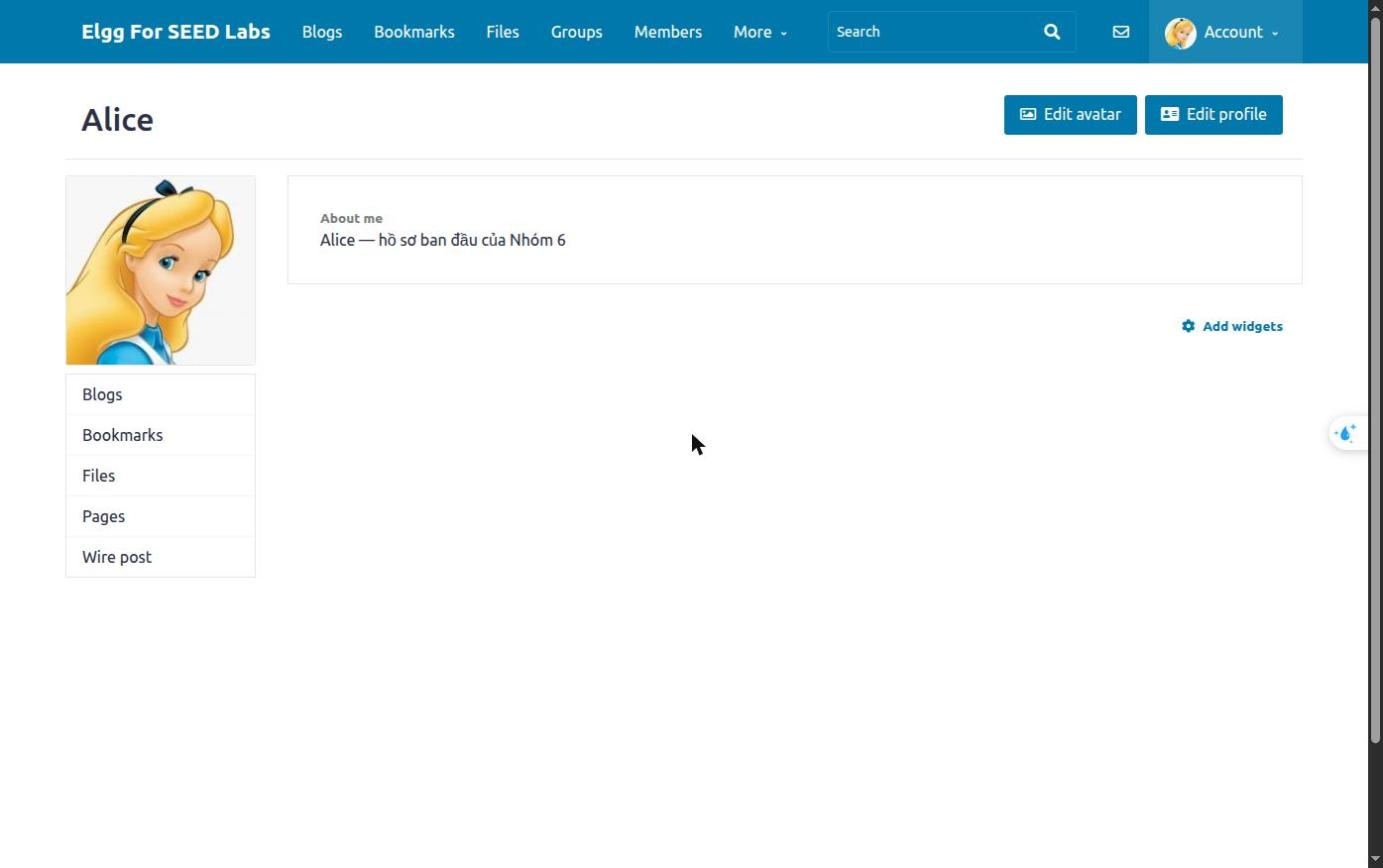
\includegraphics[width=\linewidth]{img/ev-before.jpg}}
  \\[3pt]\footnotesize\color{slate}(a) \textbf{Before:} Alice's baseline About me.
\end{minipage}\hfill
\begin{minipage}[t]{0.48\linewidth}\centering
  \fbox{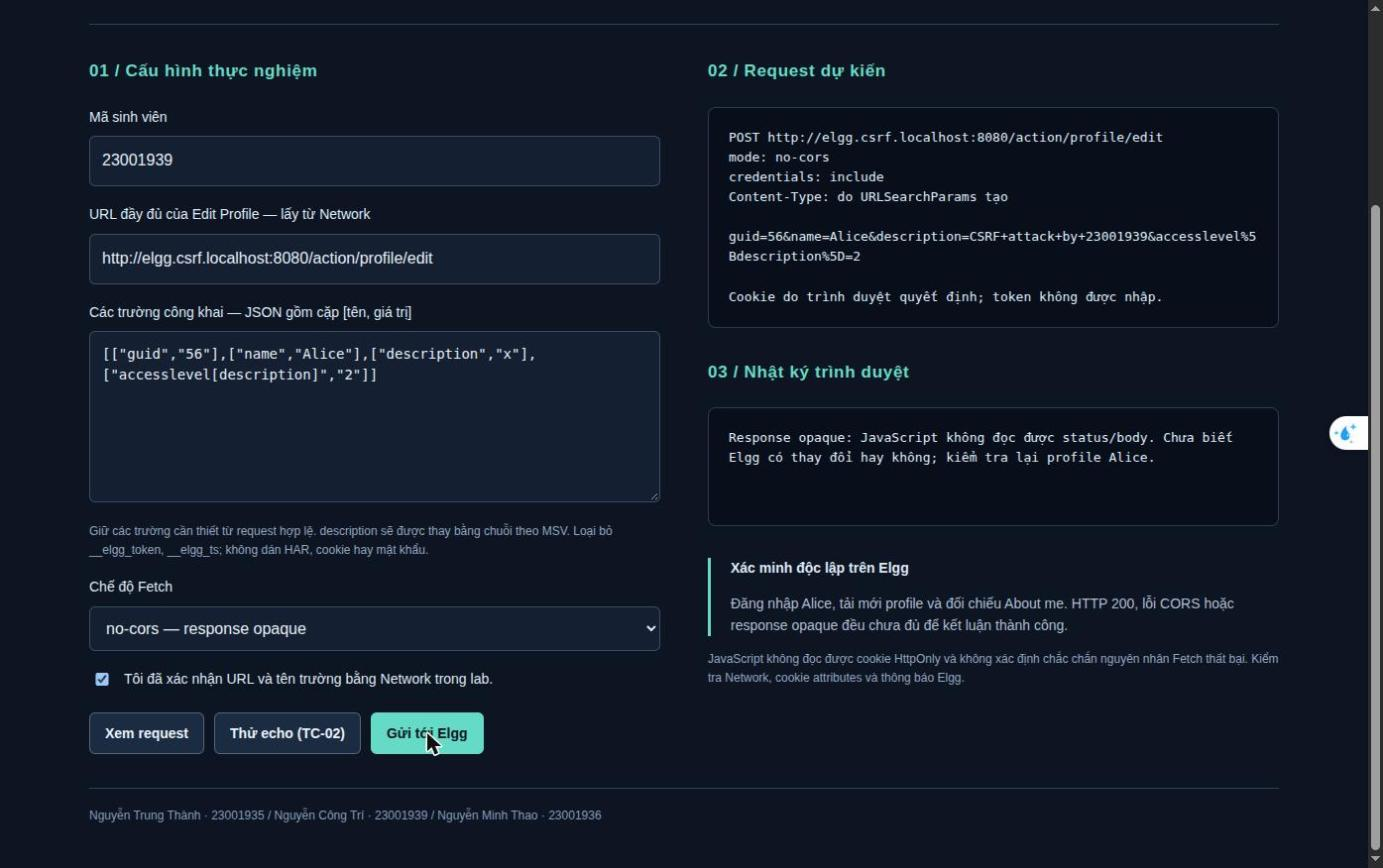
\includegraphics[width=\linewidth]{img/ev-attacker-payload.jpg}}
  \\[3pt]\footnotesize\color{slate}(b) Attacker page: the planned Fetch payload, \emph{without} a token.
\end{minipage}
\end{figure}

\begin{figure}[h]\centering
\begin{minipage}[t]{0.48\linewidth}\centering
  \fbox{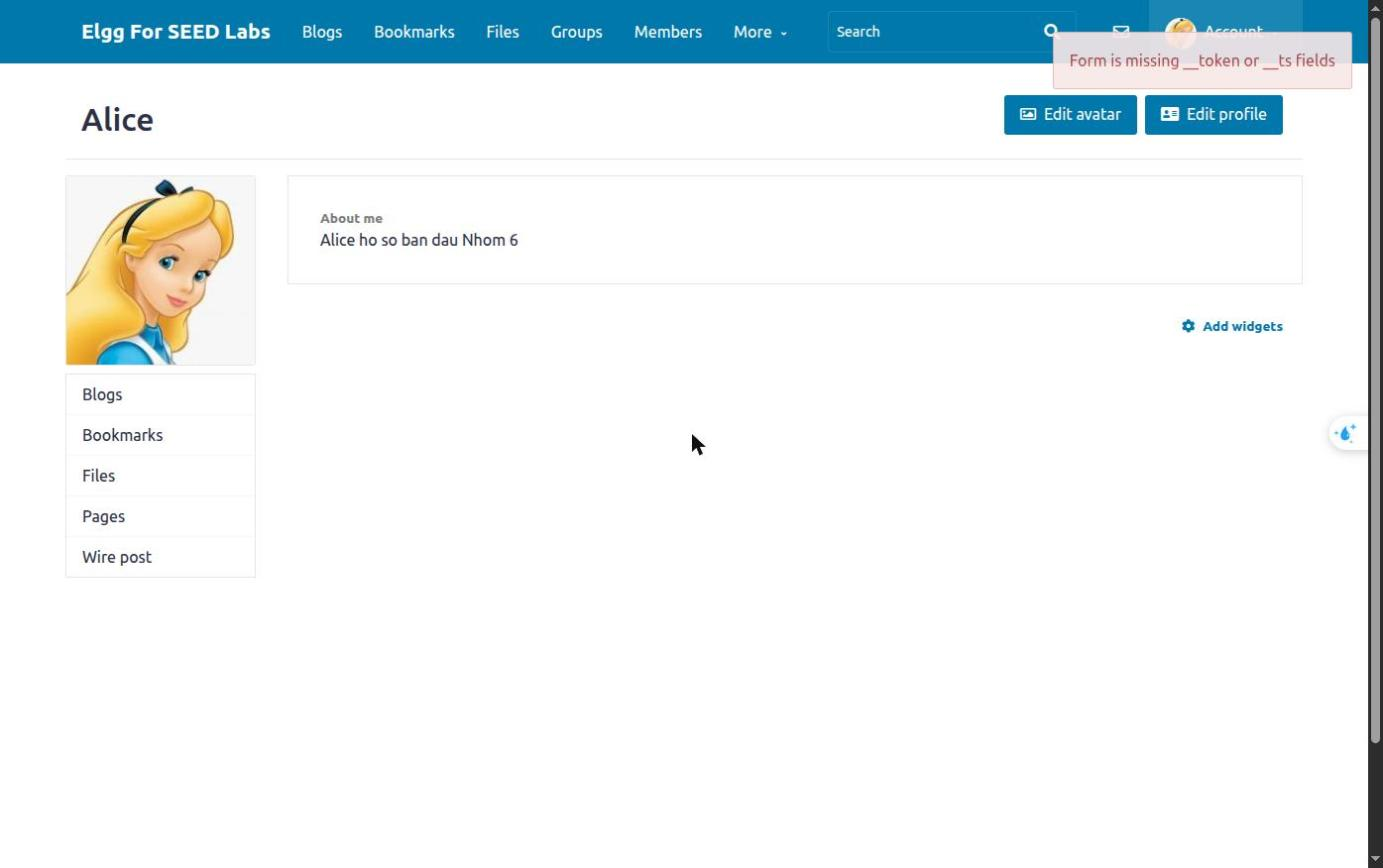
\includegraphics[width=\linewidth]{img/ev-protected-blocked.jpg}}
  \\[3pt]\footnotesize\color{slate}(c) \textbf{TC-B04 (protected):} Elgg reports \emph{``Form is missing \_\_token or \_\_ts fields''}; About me unchanged.
\end{minipage}\hfill
\begin{minipage}[t]{0.48\linewidth}\centering
  \fbox{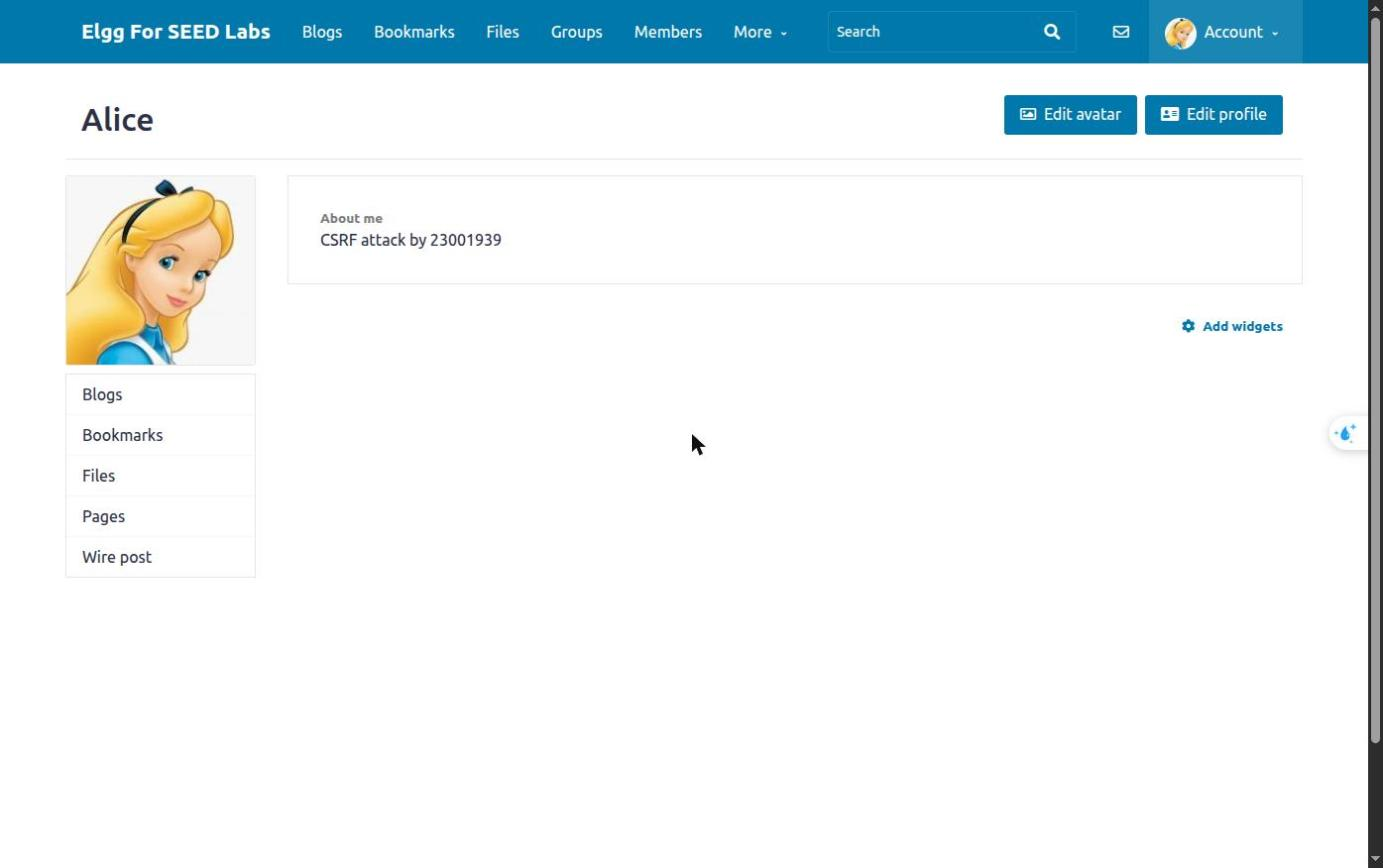
\includegraphics[width=\linewidth]{img/ev-after-success.jpg}}
  \\[3pt]\footnotesize\color{slate}(d) \textbf{TC-B06 (vulnerable, same-site):} About me = \texttt{CSRF attack by 23001939}.
\end{minipage}
\end{figure}

\begin{figure}[h]\centering
\begin{minipage}[t]{0.48\linewidth}\centering
  \fbox{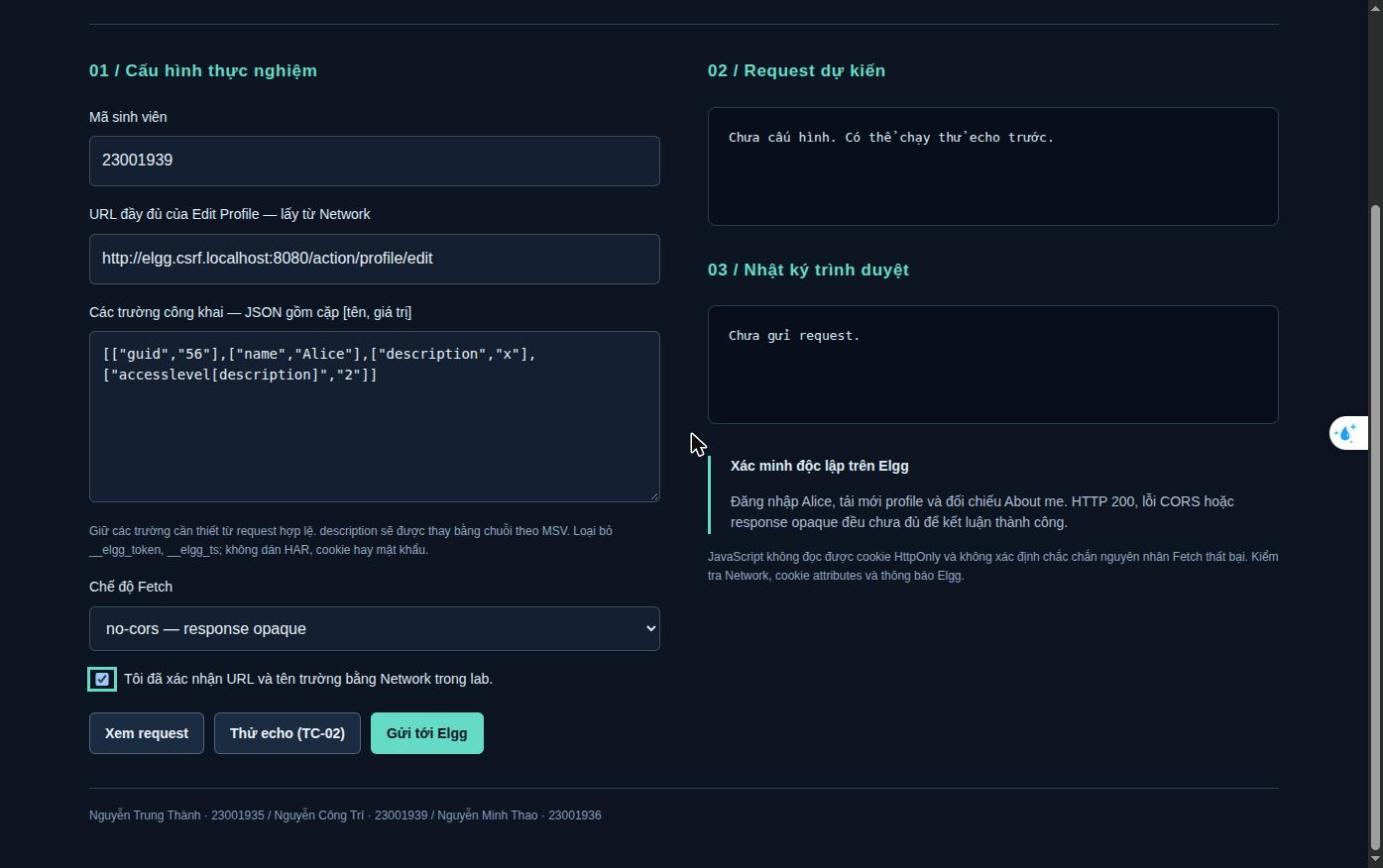
\includegraphics[width=\linewidth]{img/ev-attacker-config.jpg}}
  \\[3pt]\footnotesize\color{slate}(e) Attacker UI: configuring the endpoint + public fields (no token).
\end{minipage}\hfill
\begin{minipage}[t]{0.48\linewidth}\centering
  \fbox{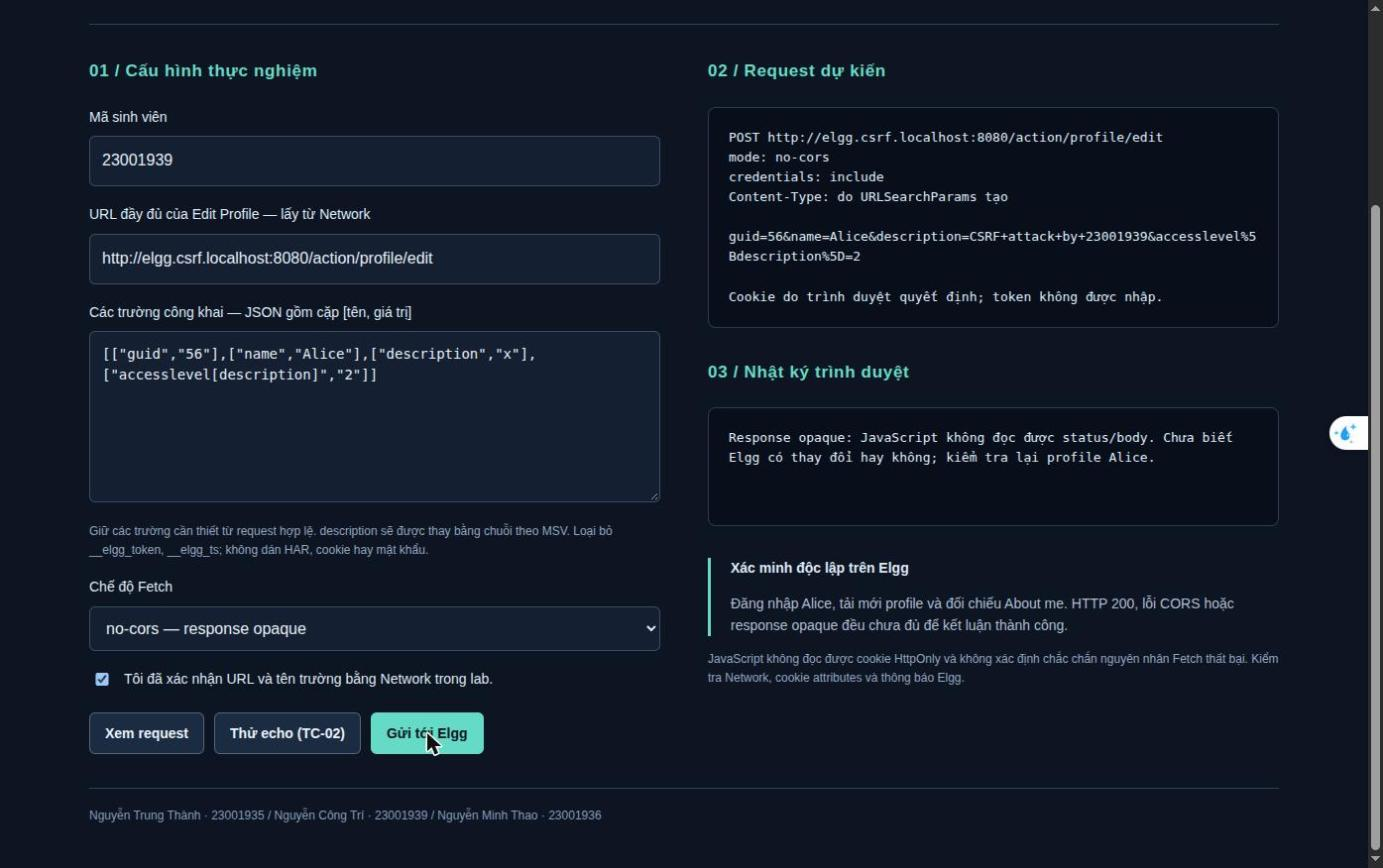
\includegraphics[width=\linewidth]{img/ev-crosssite.jpg}}
  \\[3pt]\footnotesize\color{slate}(f) \textbf{TC-B03:} attack from \texttt{127.0.0.1} (cross-site) in vulnerable mode — the profile is \emph{still} unchanged.
\end{minipage}
\end{figure}

\begin{okbox}[Core result]
In \texttt{vulnerable} mode with a same-site attacker, the About me field is changed to \texttt{CSRF attack by 23001939} with no warning or redirect — a fully successful exploit. Conversely, in \texttt{protected} mode (token on) the same payload is rejected by Elgg with a missing-token message; and in \texttt{vulnerable} but cross-site, the SameSite cookie strips the session so the profile is not changed either.
\end{okbox}

\subsection{HTTP-layer verification (curl)}
To isolate \emph{only} the token effect (curl always attaches the cookie regardless of origin, so it does not exercise SameSite), the team repeated the \emph{tokenless} POST with \texttt{curl}:
\begin{center}\small
\begin{tabularx}{\linewidth}{@{}l C C C@{}}
\toprule
\textbf{Mode} & \textbf{Tokenless POST} & \textbf{HTTP redirect} & \textbf{About me changed?}\\
\midrule
protected & blocked & $\to$ \texttt{/} (home) & \no\\
vulnerable & accepted & $\to$ \texttt{/profile/alice} & \yes\\
restored & — & — & \no\\
\bottomrule
\end{tabularx}
\end{center}
\noindent The difference in the \emph{redirect target} (home when blocked, the profile page when successful) is a clear corroborating signal, consistent with the UI observation.

\subsection{Detailed per-case narrative}
\begin{description}[leftmargin=1.6em,style=nextline]
  \item[TC-B01 — Login \& legitimate Save.] Log in as Alice, open Edit Profile, set the baseline About me, click Save. The \texttt{POST /action/profile/edit} request carries a full \texttt{\_\_elgg\_token}/\texttt{\_\_elgg\_ts}; the profile updates correctly. This is the template to mimic and the standard recovery path.
  \item[TC-B04 — Protected blocks the attack.] Keep \texttt{protected} mode. The same-site attacker page sends a POST (\texttt{credentials:'include'}, \texttt{no-cors}). The browser \emph{does} attach the cookie (same-site) but the payload \emph{lacks} the token. Elgg shows the red message \emph{``Form is missing \_\_token or \_\_ts fields''}; About me stays at baseline.
  \item[TC-B03 — SameSite blocks cross-site.] Switch to \texttt{vulnerable} (token off). Send from \texttt{127.0.0.1} (cross-site). The \texttt{SameSite} cookie makes the browser \emph{not} attach the session on a cross-site POST; Elgg treats it as a stranger so the profile is unchanged — proving SameSite protects \emph{independently} of the token.
  \item[TC-B05/06 — Successful attack.] Still \texttt{vulnerable}, send from the same-site attacker. SameSite allows the same-site cookie and the token is off $\Rightarrow$ Elgg accepts it. Reload the profile: About me = \texttt{CSRF attack by 23001939}. This is the only valid evidence (direct comparison of the displayed field).
\end{description}

% =====================================================================
\section{Technical finding: annotation vs.\ metadata}
While restoring the profile, the team discovered an important Elgg implementation detail:
\begin{itemize}
  \item The web action \texttt{/action/profile/edit} stores the About me field as an \textbf{annotation} \texttt{profile:description} (table \texttt{elgg\_annotations}) — and that is the value the \emph{profile page displays}.
  \item Meanwhile, the PHP property \texttt{\$user->description} maps to \textbf{metadata} (table \texttt{elgg\_metadata}).
\end{itemize}
\textbf{Consequence:} the \texttt{reset-profile} tool initially reset only the \emph{metadata}, so although it reported ``success'' the page still displayed the attack string; clearing the cache (\texttt{elgg-cli flush}), restarting the container or deleting the Stash cache did \emph{not} help, because the data lives in the \emph{annotation}. The correct recovery is to re-edit About me \emph{through the Edit Profile UI} (going through the proper action, overwriting the annotation), or to directly update the \texttt{profile:description} annotation.

\begin{infobox}[Lesson]
When verifying a result, one must inspect the \emph{data source the UI actually displays}. A ``successful'' change at the DB layer but in the wrong table still yields a wrong displayed result. This finding also restates that a CORS error or an opaque response is \emph{not} evidence — only a direct comparison of the displayed field is valid evidence.
\end{infobox}

% =====================================================================
\section{Verification and defenses}\label{sec:defense}
\subsection{Re-enabling Elgg's anti-CSRF token}
After restoring the \texttt{\_\_elgg\_token}/\texttt{\_\_elgg\_ts} check, re-run the exact same payload:
\begin{center}\small
\begin{tabularx}{\linewidth}{@{}Y C C@{}}
\toprule
 & \textbf{Defense OFF} & \textbf{Defense ON}\\
\midrule
Payload has \texttt{\_\_elgg\_token}? & No & Still no\\
Server response & DB updated (302) & \textbf{Rejected} (missing token)\\
Alice's About me & Changed & \textbf{Unchanged}\\
\bottomrule
\end{tabularx}
\end{center}
\noindent Because SOP forbids the attacker page's JavaScript from reading the token on the Elgg page, the forged request always lacks a valid token $\Rightarrow$ it is blocked. This is a vivid demonstration of the \emph{Synchronizer Token Pattern}.

\subsection{The independent role of the SameSite cookie}
Experiment TC-B03 shows: \emph{even when} the token is disabled (\texttt{vulnerable}), a POST from the \textbf{cross-site} attacker (\texttt{127.0.0.1}) \emph{still} cannot change the profile — because the browser does not attach the session cookie to a cross-site request (the \texttt{SameSite} cookie). Elgg treats the request as a stranger and does not act on Alice's behalf. Thus \textbf{each layer} (token or SameSite), on its own, suffices to block this attack.

\subsection{Defense-in-Depth}
\begin{center}\small
\begin{tabularx}{\linewidth}{@{}l Y Y@{}}
\toprule
\textbf{Layer} & \textbf{Measure} & \textbf{What it blocks}\\
\midrule
Cookie & \texttt{SameSite=Lax/Strict} & Browser does not send the cookie cross-site\\
Application & Anti-CSRF token (Synchronizer) & Attacker cannot read the token (thanks to SOP)\\
Application & Double Submit Cookie & Attacker cannot read the cookie to place in the body\\
Header & \texttt{Origin} / \texttt{Sec-Fetch-Site} check & Reject state-changing requests from unknown sources\\
UI & \texttt{X-Frame-Options} / CSP \texttt{frame-ancestors} & Prevent Clickjacking via iframe\\
\bottomrule
\end{tabularx}
\end{center}

\subsubsection{How each layer works}
\begin{itemize}
  \item \textbf{SameSite cookie:} enforced by the \emph{browser}. \texttt{Strict} blocks the cookie for any request originating from another site; \texttt{Lax} (today's default) still sends the cookie for top-level navigation (typing a link, clicking) but blocks it for background cross-site POSTs — just enough to stop CSRF without breaking UX. \emph{Limitation:} does not protect against a \emph{same-site} attack (e.g.\ a hijacked subdomain).
  \item \textbf{Anti-CSRF token (Synchronizer):} enforced by the \emph{server}. The server embeds a per-session random token into each form; a valid request must return the correct token. Thanks to SOP, a different-origin attacker cannot read the token. \emph{Limitation:} requires token lifecycle management; does not stop XSS.
  \item \textbf{Double Submit Cookie:} the server sends the token via both a cookie and a hidden field, then compares them — no server-side state needed. \emph{Limitation:} weak if the attacker can write the cookie (e.g.\ via a subdomain).
  \item \textbf{\texttt{Origin}/\texttt{Sec-Fetch-Site} check:} the server rejects state-changing requests from unknown sources. Simple, effective for modern APIs. \emph{Limitation:} some proxies/configurations may strip the header.
\end{itemize}

\begin{infobox}[Practical recommendation]
Combine \texttt{SameSite=Lax} (the default layer) + an anti-CSRF token (the application layer) + an \texttt{Origin} check for sensitive endpoints. Never use \texttt{GET} for a state-changing action. The \emph{defense-in-depth} principle: if one layer fails, the others still block the attack.
\end{infobox}

% =====================================================================
\section{Automated testing and reproducibility}
Beyond the manual experiment, the team maintains an automated test suite to ensure the payload is well-formed and the environment is healthy:
\begin{center}\small
\begin{tabularx}{\linewidth}{@{}Y l c@{}}
\toprule
\textbf{Test suite} & \textbf{Content} & \textbf{Result}\\
\midrule
\texttt{test\_request\_format.mjs} (Node) & 6 tests building the Fetch payload; reject token/cookie input & \yes{} 6/6\\
\texttt{test\_environment.py} & 4 tests of the attacker server: echo, static allowlist, no cookie leak & \yes{} 4/4\\
\texttt{test\_security\_controls.py} (live) & services healthy; Elgg has no CORS allowance & \yes{} 2/2\\
\texttt{docker compose config} & compose syntax check & \yes\\
\bottomrule
\end{tabularx}
\end{center}

\begin{lstlisting}[language=bash,caption={Lab reproduction procedure (summary)}]
python3 lab/scripts/labctl.py up         # bring up Elgg + MySQL + attacker
python3 lab/scripts/labctl.py version    # verify Elgg 3.3.3
# ... log in as Alice, capture request, configure attacker, try sending ...
python3 lab/scripts/labctl.py mode vulnerable   # disable token (deliberate)
python3 lab/scripts/labctl.py mode protected    # re-enable token
python3 lab/scripts/labctl.py reset-profile     # restore About me
\end{lstlisting}

% =====================================================================
\section{Task allocation}
\begin{center}\small
\begin{tabularx}{\linewidth}{@{}l l Y@{}}
\toprule
\textbf{Member} & \textbf{ID} & \textbf{Focus}\\
\midrule
Nguyen Trung Thanh & 23001935 & CSRF theory, HTTP request analysis, defenses\\
Nguyen Cong Tri & 23001939 & Elgg, Docker, Fetch API code, testing\\
Nguyen Minh Thao & 23001936 & Evidence, slides, video\\
\bottomrule
\end{tabularx}
\end{center}
\noindent \textbf{Mandatory common baseline (100\% of members):} each member runs Docker themselves, captures the request themselves and changes About me to their own student ID; all take part in the cross-examination of 15 questions.

% =====================================================================
\section{AI-usage disclosure}
\begin{enumerate}
  \item \textbf{Level 1 — Critique:} used AI to discuss \texttt{credentials: 'include'}, Simple Request and CORS; students wrote the code themselves.
  \item \textbf{Level 2 — Co-creation:} students designed the report/slide/diagram structure, AI helped polish wording and LaTeX formatting.
  \item \textbf{Level 3 — Prompted generation:} AI helped scaffold the \texttt{labctl}/attacker tooling and drive the test automation; students configured the real values, ran them and own the results.
\end{enumerate}
\noindent All experimental results and their accuracy are the direct responsibility of the team.

% =====================================================================
\section{Discussion, limitations and future work}
\subsection{What was achieved}
\begin{itemize}
  \item A real end-to-end run on the Chrome browser with Elgg 3.3.3; visual evidence of all three states (before / blocked / success).
  \item Rigorous variable control to \emph{isolate} the roles of the anti-CSRF token and the SameSite cookie.
  \item Strict adherence to ethics: no token/cookie entered into the attacker; the tool actively rejects secret fields.
\end{itemize}
\subsection{Limitations}
\begin{itemize}
  \item The standard SEED model (\texttt{www.seed-server.com}) is presented only conceptually; all evidence comes from the team's local Docker lab.
  \item Disabling the token is a \emph{deliberate} lab modification for illustration, not a conclusion that the current Elgg release is flawed.
  \item A \texttt{no-cors} response is opaque so the status code cannot be read from JS; conclusions rely solely on direct profile comparison (handled correctly).
\end{itemize}
\subsection{Future work}
\begin{itemize}
  \item Add an \emph{add friend} attack scenario (only the victim's own guid needed) to compare with the profile-edit scenario.
  \item Experiment with different \texttt{SameSite} values (\texttt{Strict}/\texttt{Lax}/\texttt{None}) and directly observe cookie attach/strip in the Network tab.
  \item Fix the \texttt{reset-profile} tool to reset the correct \texttt{profile:description} annotation.
\end{itemize}

% =====================================================================
\section{Conclusion}
The team achieved the objective: changed About me to \texttt{CSRF attack by 23001939} via the Fetch API (no XHR/Form), fully analysed the exploitation mechanism, \emph{actually ran} it on the Docker lab (Elgg 3.3.3) with visual evidence, and \emph{experimentally proved} the effectiveness of two independent defense layers (anti-CSRF token and SameSite cookie). The core lesson: CSRF is not prevented by HTTPS; the fundamental remedy is the \texttt{SameSite} cookie combined with an anti-CSRF token and request-origin checking. The annotation/metadata finding also stresses a principle: conclude only from directly compared evidence, never from indirect signals.

% =====================================================================
\appendix
\section{Appendix A: Answers to the 15 questions (summary)}
\small
\begin{enumerate}[leftmargin=2.2em]
\item \textbf{SameSite stops CSRF:} instructs the browser not to send the cookie on cross-site requests (Strict/Lax) $\Rightarrow$ the forged request loses its authenticated session.
\item \textbf{Secret token:} the server embeds a per-session random token into the form; thanks to SOP the attacker cannot read it $\Rightarrow$ a forged tokenless request is rejected.
\item \textbf{HTTPS still worries about CSRF:} HTTPS only secures transport; the cookie is still attached inside the TLS tunnel, so CSRF (an application-layer flaw) is not prevented.
\item \textbf{GET \texttt{delete.php?pageid=5}:} use a hidden \texttt{<img src=...>} or \texttt{fetch(...,\{credentials:'include'\})} to trigger the forged GET.
\item \textbf{POST \texttt{delete.php}:} use Fetch + \texttt{URLSearchParams(pageid=5)}, running silently with no page change.
\item \textbf{Finding Boby's guid:} via the profile URL, avatar \texttt{src}, the Add-friend link, or the RSS feed — all public.
\item \textbf{Unknown user id:} depends on the server — if the id is derived from the session the attack still works; if a large random id must be in the body, it does not.
\item \textbf{Attacking an arbitrary guest:} (1) \no{} editing a profile — needs the victim's guid that SOP forbids reading; (2) \yes{} add friend — only needs Alice's own guid, the victim's identity is derived from the session.
\item \textbf{Session ID in the data part (Double Submit):} the cookie is auto-sent by the browser, but the data part must be set by the origin page's JS; the attacker cannot read the cookie so cannot fill it correctly $\Rightarrow$ the server detects the cross-site forgery.
\item \textbf{Does the browser know cross-site?} Yes — it knows the source and destination origins, sends \texttt{Origin}, \texttt{Sec-Fetch-Site}.
\item \textbf{Does the server know cross-site?} By default with plain HTTP, no; it can know if it checks \texttt{Origin}/\texttt{Referer}/\texttt{Sec-Fetch-Site}/token.
\item \textbf{Why not rely on Referer alone:} the Referer may be legitimately dropped (\texttt{Referrer-Policy}, HTTPS→HTTP, proxy) and is easy to bypass with loose regex.
\item \textbf{Why we need to know cross-site:} to allow a state-changing action only when the user genuinely intends it, avoiding borrowed authority.
\item \textbf{Ban cross-site cookies entirely?} Technically possible but it breaks navigation, SSO/OAuth and embedded widgets; the solution is \texttt{SameSite=Lax} by default.
\item \textbf{Facebook iframe:} a request from within an iframe to Facebook is same-site with respect to Facebook (not cross-site); the risk is Clickjacking; mitigate with \texttt{X-Frame-Options} / CSP \texttt{frame-ancestors}.
\end{enumerate}

\section{Appendix B: Reproduction details}
\small
\begin{itemize}
  \item \textbf{Versions:} Elgg 3.3.3 (digest \texttt{sha256:5d8a25b1\ldots708f7f5}); MySQL 8.0.37; attacker Python 3.12.
  \item \textbf{Public SEED accounts (lab-only):} Alice \texttt{alice}/\texttt{seedalice}; admin \texttt{admin}/\texttt{seedelgg}.
  \item \textbf{Target string:} \texttt{CSRF attack by 23001939} (change per student ID in \texttt{.env} or the attacker UI).
  \item \textbf{Recovery:} \texttt{labctl mode protected} + re-edit About me to baseline through the Edit Profile UI.
\end{itemize}

\begin{thebibliography}{9}\small
\bibitem{du} W. Du, \emph{Computer \& Internet Security: A Hands-on Approach}, 3rd ed.
\bibitem{fetch} WHATWG, \emph{Fetch Living Standard}, \url{https://fetch.spec.whatwg.org/}.
\bibitem{owasp} OWASP, \emph{Cross-Site Request Forgery Prevention Cheat Sheet}.
\bibitem{samesite} IETF, \emph{RFC 6265bis — Cookies: SameSite attribute}.
\bibitem{elgg} Elgg, \emph{Actions \& Security}, \url{https://learn.elgg.org/}.
\end{thebibliography}

\end{document}
